%!TEX root = ./template-skripsi.tex
%-------------------------------------------------------------------------------
% 								BAB I
% 							LATAR BELAKANG
%-------------------------------------------------------------------------------

\chapter{PENDAHULUAN}

\section{Latar Belakang Masalah}

Saat ini, penggunaan \textit{search engine} atau mesin pencari telah digunakan oleh khalayak umum untuk mencari berbagai informasi yang ada. Berdasarkan data dari \citep{reliablesoft2022}, Google merupakan \textit{search engine} yang menempati urutan pertama terpopuler, selanjutnya diikuti dengan Bing, Baidu, Yahoo!, Yandex, dan DuckDuckGo.

\begin{figure}[h]
    \centering
    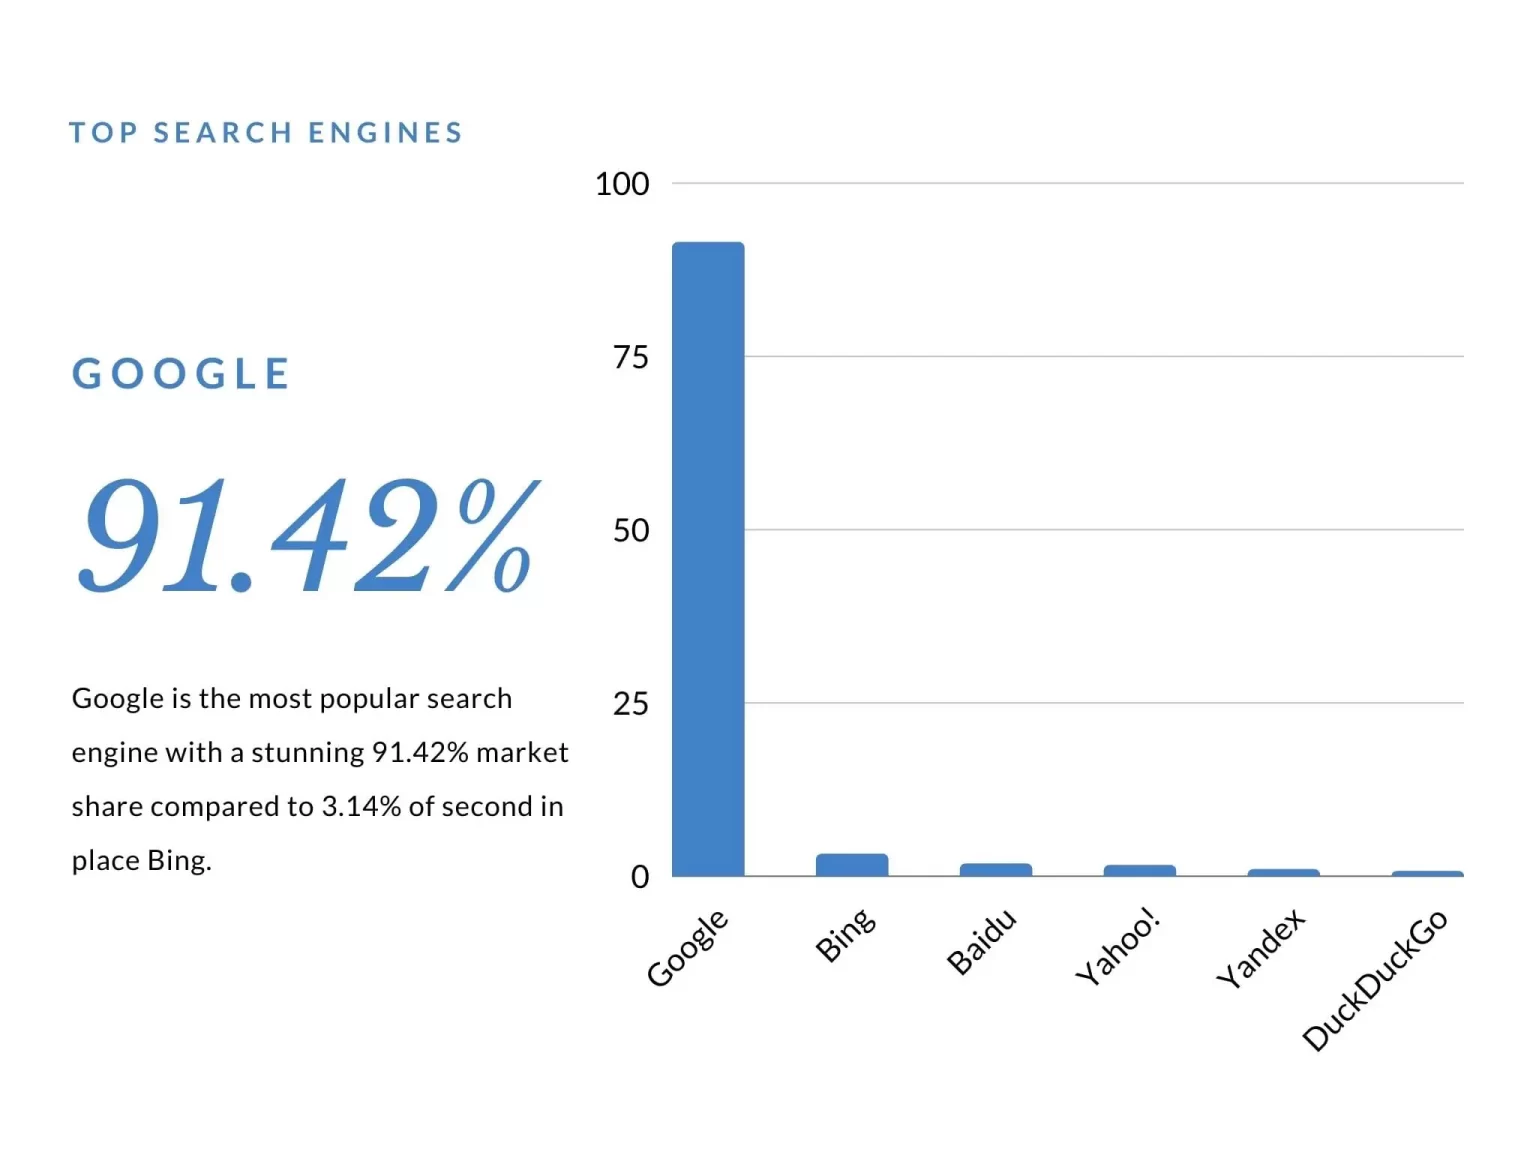
\includegraphics[width=0.75\textwidth]{gambar/Top Search Engine.png}
    \caption{Pengguaan search engine terpopuler \citep{reliablesoft2022}}
    \label{gambar:search_engine_populer}
\end{figure}

\textit{Web Search Engine} atau mesin pencari web merupakan suatu perangkat lunak yang digunakan untuk mencari sesuatu di internet berdasarkan kata-kata yang diberikan oleh pengguna sebagai \textit{search terms}. Pembuatan \textit{search engine} pertama kali dilakukan oleh Alan Emtage, Bill Heelan, dan J. Peter Deutsch pada tahun 1990. Mereka menamai \textit{search engine} tersebut yaitu Archie \citep{seymour2011history}.

Pekerjaan utama dari \textit{search engine} ada tiga yaitu \textit{web crawling, indexing,} dan \textit{searching}. \textit{Search engine} bekerja dengan cara mengirimkan informasi tentang halaman web, Halaman tersebut di dapat dari \textit{web crawler} suatu \textit{automated web browser} yang mengikuti seluruh pranala yang ada di situs. Pengecualian situs yang dicari dapat dilakukan melalui "\textit{robots.txt}". Kemudian, konten dari setiap halaman akan dianalisis untuk menentukan urutan index. Data tentang halaman web dikirim ke dalam \textit{index database} yang nantinya akan dilakukan \textit{query}. \textit{Query} bisa satu kata atau lebih. Tujuan pengindeksan adalah untuk menemukan informasi secepat mungkin \citep{seymour2011history}.

\begin{figure}[h]
    \centering
    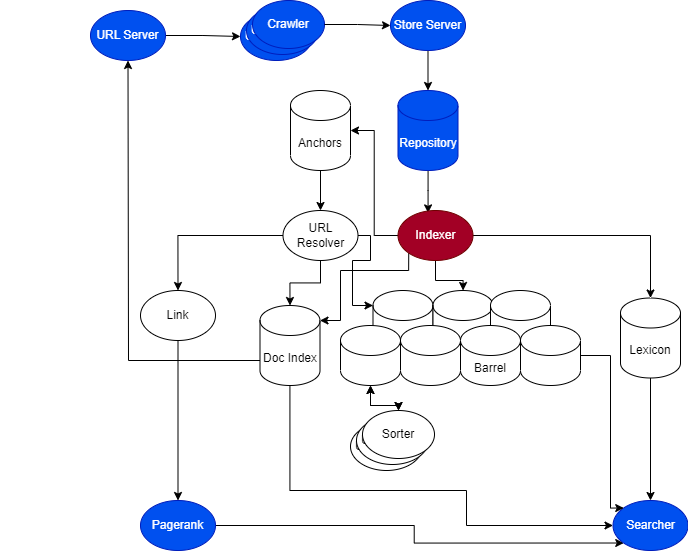
\includegraphics[width=0.75\textwidth]{gambar/Skema Search Engine Google.png}
    \caption{High Level Google Architecture \citep{brin1998anatomy}}
    \label{gambar:high_level_google_architecture}
\end{figure}

Pada Gambar \ref{gambar:search_engine_populer}, telah diperlihatkan bahwa Google merupakan \textit{search engine} terfavorit. Google ditemukan oleh Larry Page dan Sergey Brin pada tahun 1998. Salah satu keunggulan Google adalah pengaplikasian PageRank  yaitu mengatasi \textit{underspecified queries}. Sebagai contohnya, jika kita mencari kata Real Madrid, maka situs pertama kali yang terlihat adalah situs resmi Real Madrid.

Gambar \ref{gambar:high_level_google_architecture} merupakan struktur arsitektur Google. Warna biru menunjukkan hasil penelitian yang dilakukan oleh Lazuardy Khatulistiwa dalam penelitian yang berjudul “Perancangan Arsitektur Search Engine dengan Mengintegrasikan \textit{Web Crawler, Algoritma Page Ranking}, dan \textit{Document Ranking}” dan warna merah menunjukkan proses penelitian dari Zaidan Pratama dalam judul “Perancangan Modul Pengindeks pada \textit{Search Engine} Berupa \textit{Induced Generalized Suffix Tree} untuk Keperluan Perangkingan Dokumen”.
Salah satu komponen dalam \textit{search engine} milik Google adalah \textit{Indexer}. Dalam penelitian Zaidan Pratama, di sana menjelaskan tentang melakukan pengindeksan melalui algoritma \textit{General Suffix Tree} (\textit{GST}) yang termodifikasi. (\cite{pratama2022igst})

% Akan tetapi, penelitian ini memiliki kekurangan yaitu hanya bisa mengambil judul dari suatu dokumen. Beberapa dokumen terkadang tidak memiliki relevansi dengan judulnya dan itu bisa saja menyebabkan masalah sehingga diperlukan adanya tag.

Proses pengindeksan dimulai dengan memasukkan kumpulan dokumen yang dibuat menjadi \textit{GST}. Kemudian, membuat \textit{GST} dari kumpulan dokumen tersebut. Dari \textit{GST} tersebut, nantinya akan dilakukan reduksi untuk node yang redundan atau node yang mengalami perulangan yang tidak diperlukan sehingga akan terbentuk pohon yang terinduksi untuk frekuensi \textit{f} yang bernama \textit{Induced Generalized Suffix Tree-f}. 

\textit{IGST-f}  ini menjadi komponen utama dalam pengindeksan. Setelah itu, program menerima masukan berupa pola kata dan batas \textit{k} untuk dicari pada kumpulan dokumen. Dari sinilah kita akan mencari nilai \textit{count} dari setiap \textit{node}. Kemudian, mencatat jumlah dokumen dalam \textit{sublist} yang tereduksi untuk setiap \textit{node}. Selanjutnya, mencari nilai \textit{counter lowest common ancestor} dari setiap \textit{node}. Terakhir, mengenai Indeks Efisien. Untuk \textit{Top-k Document Retrieval Problem} dilakukan pengurutan terhadap representasi \textit{array IGST-f} yang sudah memiliki nilai \textit{count} dan mengembalikan hasil \textit{top-k} yang meiliki pola \textit{P}. \cite{pratama2022igst}

\begin{figure}[H]
    \centering
    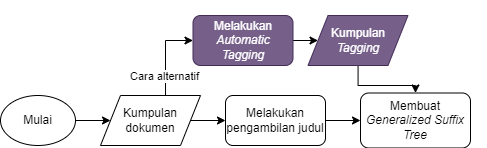
\includegraphics[width=1\textwidth]{gambar/Skema singkat General Suffix Tree.png}
    \caption{Bagian \textit{Automatic Tagging} pada \textit{Indexer}}
    \label{gambar:automatic_tagging}
\end{figure}

Akan tetapi, pengindeksan tersebut masih hanya melalui judul dan belum melalui \textit{tag}. Oleh karena itu, salah satu alternatifnya adalah melakukan pengindeksan melalui \textit{tag}. Pada gambar \ref{gambar:automatic_tagging} Warna ungu adalah salah satu alternatif yang dapat dilakukan yaitu melalui \textit{automatic tagging} yang nantinya peneliti akan lakukan. Hal ini dapat dimanfaatkan agar bisa melakukan pengindeksan lebih akurat.
	
\textit{Tagging} merupakan hal yang biasa dilakukan untuk menggambarkan suatu kata kunci yang relevan atau frasa kunci pada suatu dokumen, gambar, atau video. Dalam merambatnya perkembangan Web 2.0 aplikasi seperti Del.icio.us dan Flickr, pelayanan \textit{tagging} mulai populer dan menarik perhatian pihak akademis dan industri. Penelitian tentang cara \textit{automatic tag} membuahkan hasil. Cara melakukannya dengan algoritma \textit{Poisson Mixture Model}. Dengan cara ini, kecepatan untuk membuat \textit{automatic tag} bisa lebih cepat dibandingkan SimFusion dan VS+IG. Contohnya pada saat \textit{Delicious Test Time}, \textit{PMM} mampu menghasilkan 1,23 detik saat proses \textit{automatic tag}, sedangkan SimFusion membutuhkan waktu 6,4 detik dan \textit{VS+IG} membutuhkan waktu 77,43 detik. Selain kecepatan, \textit{PMM} juga mampu di atas \textit{SimFusion} serta \textit{VS+IG} secara signifikan dalam hal akurasi, presisi, dan \textit{recall}. \citep{song2008autotag}

Selain itu, \textit{tagging} juga digunakan untuk membantu pengorganisasian, \textit{browsing}, dan pencarian. Seperti \textit{image tagging} yang digunakan oleh Flickr, \textit{web page tagging} yang digunakan oleh Del.ico.us, dan \textit{social tagging} yang digunakan oleh Facebook, semua sistem tersebut menjadi populer dan dipergunakan di penjuru Web. \citep{sood2007tagassist}

Secara umum, sumber yang memiliki \textit{tag} biasanya berasosiasi \textit{tag} yang lain. Selain itu, sumber yang memiliki \textit{tag} berasosiasi terhadap \textit{user}. Sebagai contoh, \textit{tagging} terhadap dokumen $d$ yang dilakukan oleh \textit{user} $u$ dengan \textit{tag} $t$ dapat direpresentasikan sebagai tiga kesatuan $(u, d, t)$. Dengan menggunakan pendekatan itu, dapat terbentuk suatu graf yang digambarkan sebagai berikut. 

\begin{figure}[h]
    \centering
    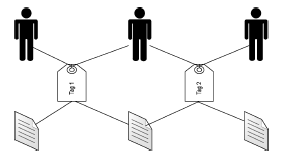
\includegraphics[width=0.75\textwidth]{gambar/skema automatic tag.PNG}
    \caption{Relasi antara user, tag, dan dokumen \citep{song2011autotag}}
    \label{gambar:relasi_user_tag_dokumen}
\end{figure}

Dengan relasi pada gambar \ref{gambar:relasi_user_tag_dokumen} , rekomendasi \textit{tag} dapat dilakukan dengan dua jenis menurut Song yaitu jenis pendekatan melalui pengguna dan jenis pendekatan melalui dokumen. Rekomendasi \textit{tag} merupakan suatu sistem yang di mana sistem tersebut menampilkan \textit{tag} yang relevan pada suatu dokumen agar pengguna bisa memperhitungkan apakah \textit{tag} yang ditampilkan itu ingin dipakai atau tidak. Melalui pendekatan \textit{user}, sistem ini akan mengolah rekomendasi \textit{tag} berdasarkan \textit{tag-tag} yang telah dilakukan \textit{user} sebelumnya dan merekomendasikan tag yang mirip dengan \textit{user} ini atau kelompok dari \textit{user} tersebut. Berbeda halnya dengan pendekatan dokumen, cara ini dilakukan dengan cara mengklasterisasikan dokumen-dokumen tersebut ke dalam topik-topik yang berbeda. Topik yang sama pada suatu dokumen akan memiliki \textit{tag} yang diasumsikan lebih mirip dibandingkan dokumen yang berbeda topik. Namun, di antara kedua cara ini, yang dinilai kurang efektif adalah melalui pendekatan \textit{user}. Pertama, berdasarkan penelitian dari \cite{farooq_social_bookmarking}, distribusi dari \textit{user} vs \textit{tag} mengikuti \textit{long tail power law distribution}. Itu artinya, hanya sebagian kecil porsi dari \textit{user} yang melakukan \textit{tag} dengan panjang atau meluas. Sebagai tambahan, penggunaan \textit{tag} yang berulang juga terbilang rendah, tetapi pertumbuhan perbendaharaan \textit{tag} terus berkembang. Dengan sedikit pengguna relatif yang didapat, pendekatan \textit{user} akan sulit untuk mencari model mana yang cocok buat untuk melakukan rekomendasi \textit{tag} yang efektif. Berbanding terbalik dengan pendekatan dokumen yang lebih kokoh karena kekayaan informasi yang ada di dokumen. Bahkan, \textit{tag} dan kata akan menciptakan relasi yang potensial antara topik dan konten di suatu dokumen yang di mana tag dianggap sebagai kelas label untuk dokumen dalam skenario \textit{supervised learning} atau kesimpulan dari dokumen dalam skenario \textit{unsupervised learning}. \citep{song2011autotag}

Namun, percobaan ini hanya terbatas pada CiteULike dan del.icio.us. Untuk saat ini, kedua situs tersebut sudah tidak dapat diakses dengan semestinya. CiteULike beralih menjadi situs judi, sedangkan del.icio.us tidak dapat diakses oleh umum.
	
Beberapa tahun kemudian, suatu penelitian membahas mengenai \textit{automatic mashup tag}. Secara sederhana, \textit{mashup} adalah suatu \textit{web service} yang di mana merupakan kumpulan dari kombinasi beberapa Web \textit{API} dan konten dari berbagai sumber. Berbeda dengan rekomendasi \textit{tag} yang menggunakan pendekatan dengan konten tekstual, di dalam \textit{Web services} terdapat banyak sekali relasi seperti komposisi relasi antara \textit{mashup} dengan \textit{API} dan anotasi berelasi antara \textit{API} dan \textit{tag}. \citep{shi2016mashuptag}

\begin{figure}[H]
    \centering
    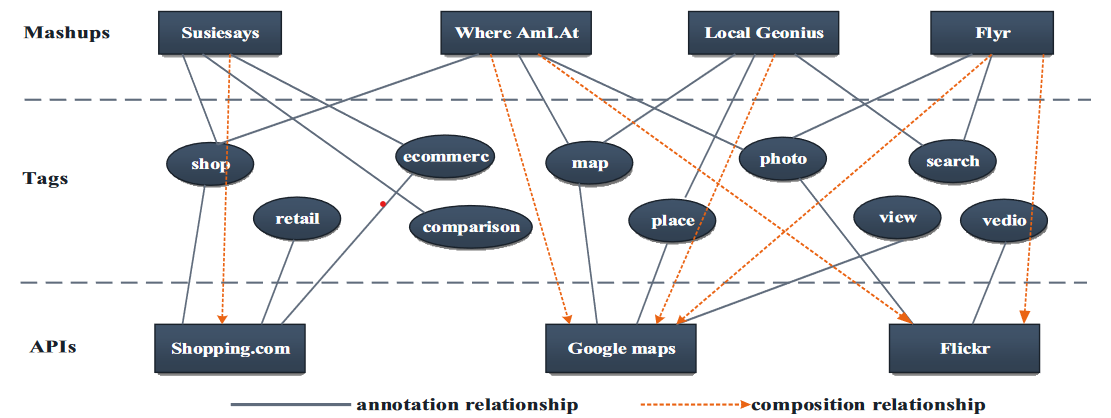
\includegraphics[width=1\textwidth]{gambar/mashup tag api.PNG}
    \caption{Skema \textit{Mashup}, \textit{Tag}, dan \textit{API} \citep{shi2016mashuptag}}
    \label{gambar:mashup_tag_api}
\end{figure}

Selain teks, \textit{tag} juga digunakan dalam hal yang bersifat non teks seperti video, musik, dan gambar. Dalam suatu video, \textit{tag} sangat diperlukan untuk menentukan relevansi antara pencarian yang diinginkan dengan isi video. Meskipun beberapa platform video seperti Youtube menyediakan judul dan deskripsinya, bisa saja judul tersebut tidak ada keterkaitannya dengan video dan deskripsinya yang sangat panjang sehingga orang malas untuk membaca. Manfaat dalam \textit{tag} video ada dua yaitu bisa menemukan daftar video yang representatif dan \textit{tag} dapat mendukung untuk melakukan penemuan tentang video yang kontennya berhubungan dengan video yang telah ditonton. \citep{parra2018videotag}

Untuk kasus \textit{automatic tag} pada musik, \textit{Automatic music tagging} adalah \textit{multi label binary classification} yang bertujuan untuk memprediksi \textit{tag} yang relevan pada suatu lagu. \textit{Tag} tersebut membawa informasi musik semantik yang nantinya dapat digunakan untuk membuat aplikasi seperti rekomendasi musik. \citep{won2020musictag}

Dengan demikian, peneliti ingin membuat penelitian terkait \textit{automatic tagging} dengan menggunakan penelitian dari \cite{song2008autotag} yang terdapat dua algoritma utama yaitu \textit{Bipartite Graph Partition} dan \textit{Two Way Poisson Mixture Model}.

\section{Rumusan Masalah}

Berdasarkan  latar belakang masalah yang telah diuraikan, maka perumusan masalah pada penelitian ini adalah "Bagaimana cara melakukan Automatic Tagging dengan menggunakan algoritma \textit{Bipartite Graph Partition} dan \textit{Two Way Poisson Mixture Model}?".

\section{Batasan Masalah}

Batasan masalah dalam penelitian ini yaitu:

\begin{enumerate}
    \item Data latih dan data uji yang digunakan berasal dari satu sumber \textit{web}.
    \item Untuk \textit{crawling} data, akan digunakan \textit{crawler} dari sistem yang telah dibuat oleh \cite{khatulistiwa_2022_searchengine} berjudul "Perancangan Arsitektur Search Engine dengan Mengintegrasikan Web Crawler, Algoritma Page Ranking, dan Document Ranking".
    \item Banyaknya $K$ yang digunakan adalah dua.
\end{enumerate}

\section{Tujuan Penelitian}

Tujuan dari penelitian ini adalah untuk membuat program \textit{automatic tagging} dengan menggunakan algoritma \textit{Bipartite Graph Partition} dan \textit{Two Way Poisson Mixture Model} sesuai penelitian \cite{song2008autotag}.

\section{Manfaat Penelitian}

Dalam penelitian ini, manfaat yang bisa diperoleh yaitu:

\begin{enumerate}
    \item Bagi Peneliti
    \begin{itemize}
        \item[] Menambah pengetahuan penulis tentang \textit{automatic tagging} terhadap dokumen.
    \end{itemize}
    \item Bagi Peneliti Selanjutnya
    \begin{itemize}
        \item[] Diharapkan metode yang diusulkan pada penelitian ini dapat membantu penelitian selanjutnya dalam mengembangkan sistem yang lebih kompleks dan bermanfaat.
    \end{itemize}
\end{enumerate}


% Baris ini digunakan untuk membantu dalam melakukan sitasi
% Karena diapit dengan comment, maka baris ini akan diabaikan
% oleh compiler LaTeX.
\begin{comment}
\bibliography{daftar-pustaka}
\end{comment}
